\documentclass[a4paper,11pt,twoside]{ThesisStyle}

%!TEX root = Manuscript.tex
\usepackage{array}
\usepackage{gensymb}

\usepackage{amsmath,amssymb}
\usepackage[T1]{fontenc}
\usepackage[utf8]{inputenc}
\usepackage[english]{babel}

\usepackage[left=1.5in,right=1.3in,top=1.1in,bottom=1.1in,includefoot,includehead,headheight=13.6pt]{geometry}
\renewcommand{\baselinestretch}{1.05}

\usepackage{silence}

\WarningFilter{minitoc(hints)}{W0023}
\WarningFilter{minitoc(hints)}{W0024}
\WarningFilter{minitoc(hints)}{W0028}
\WarningFilter{minitoc(hints)}{W0030}

\usepackage{aecompl}
\usepackage{url}

% List of abbreviations
% Do not try putting acronyms in section titles, that would cause infinite loop of pdftex compilation
\usepackage[printonlyused,withpage]{acronym}

% My pdf code

\usepackage{ifpdf}

\ifpdf
  \usepackage[pdftex]{graphicx}
\else
  \usepackage{graphicx}
\fi

\graphicspath{{.}{images/}}

% Links in pdf
\usepackage{color}
\definecolor{linkcol}{rgb}{0,0,0.4}
\definecolor{citecol}{rgb}{0.5,0,0}

% Table of contents for each chapter

\usepackage[nottoc, notlof, notlot]{tocbibind}
\usepackage{minitoc}
\setcounter{minitocdepth}{2}
\mtcindent=15pt
% Use \minitoc where to put a table of contents

% definitions.
% -------------------

\setcounter{secnumdepth}{3}
\setcounter{tocdepth}{2}

% Some useful commands and shortcut for maths:  partial derivative and stuff

\newcommand{\pd}[2]{\frac{\partial #1}{\partial #2}}
\def\abs{\operatorname{abs}}
\def\argmax{\operatornamewithlimits{arg\,max}}
\def\argmin{\operatornamewithlimits{arg\,min}}
\def\diag{\operatorname{Diag}}
\newcommand{\eqRef}[1]{(\ref{#1})}

\usepackage{rotating}                    % Sideways of figures & tables
%\usepackage{bibunits}
%\usepackage[sectionbib]{chapterbib}          % Cross-reference package (Natural BiB)
%\usepackage{natbib}                  % Put References at the end of each chapter
                                         % Do not put 'sectionbib' option here.
                                         % Sectionbib option in 'natbib' will do.
\usepackage{fancyhdr}                    % Fancy Header and Footer

% \usepackage{txfonts}                     % Public Times New Roman text & math font

%%% Fancy Header %%%%%%%%%%%%%%%%%%%%%%%%%%%%%%%%%%%%%%%%%%%%%%%%%%%%%%%%%%%%%%%%%%
% Fancy Header Style Options

\pagestyle{fancy}                       % Sets fancy header and footer
\fancyfoot{}                            % Delete current footer settings

%\renewcommand{\chaptermark}[1]{         % Lower Case Chapter marker style
%  \markboth{\chaptername\ \thechapter.\ #1}}{}} %

%\renewcommand{\sectionmark}[1]{         % Lower case Section marker style
%  \markright{\thesection.\ #1}}         %

\fancyhead[LE,RO]{\bfseries\thepage}    % Page number (boldface) in left on even
% pages and right on odd pages
\fancyhead[RE]{\bfseries\nouppercase{\leftmark}}      % Chapter in the right on even pages
\fancyhead[LO]{\bfseries\nouppercase{\rightmark}}     % Section in the left on odd pages

\let\headruleORIG\headrule
\renewcommand{\headrule}{\color{black} \headruleORIG}
\renewcommand{\headrulewidth}{1.0pt}
\usepackage{colortbl}
\arrayrulecolor{black}

\fancypagestyle{plain}{
  \fancyhead{}
  \fancyfoot{}
  \renewcommand{\headrulewidth}{0pt}
}

\usepackage{algorithm}
\usepackage[noend]{algorithmic}
\usepackage{scrextend}

%%% Clear Header %%%%%%%%%%%%%%%%%%%%%%%%%%%%%%%%%%%%%%%%%%%%%%%%%%%%%%%%%%%%%%%%%%
% Clear Header Style on the Last Empty Odd pages
\makeatletter

\def\cleardoublepage{\clearpage\if@twoside \ifodd\c@page\else%
  \hbox{}%
  \thispagestyle{empty}%              % Empty header styles
  \newpage%
  \if@twocolumn\hbox{}\newpage\fi\fi\fi}

\makeatother

%%%%%%%%%%%%%%%%%%%%%%%%%%%%%%%%%%%%%%%%%%%%%%%%%%%%%%%%%%%%%%%%%%%%%%%%%%%%%%%
% Prints your review date and 'Draft Version' (From Josullvn, CS, CMU)
\newcommand{\reviewtimetoday}[2]{\special{!userdict begin
    /bop-hook{gsave 20 710 translate 45 rotate 0.8 setgray
      /Times-Roman findfont 12 scalefont setfont 0 0   moveto (#1) show
      0 -12 moveto (#2) show grestore}def end}}
% You can turn on or off this option.
% \reviewtimetoday{\today}{Draft Version}
%%%%%%%%%%%%%%%%%%%%%%%%%%%%%%%%%%%%%%%%%%%%%%%%%%%%%%%%%%%%%%%%%%%%%%%%%%%%%%%

\newenvironment{maxime}[1]
{
\vspace*{0cm}
\hfill
\begin{minipage}{0.5\textwidth}%
%\rule[0.5ex]{\textwidth}{0.1mm}\\%
\hrulefill $\:$ {\bf #1}\\
%\vspace*{-0.25cm}
\it
}%
{%

\hrulefill
\vspace*{0.5cm}%
\end{minipage}
}

\let\minitocORIG\minitoc
\renewcommand{\minitoc}{\minitocORIG \vspace{1.5em}}

\usepackage{subfigure}
\usepackage{multirow}
% \usepackage{slashbox}

\newenvironment{bulletList}%
{ \begin{list}%
	{$\bullet$}%
	{\setlength{\labelwidth}{25pt}%
	 \setlength{\leftmargin}{30pt}%
	 \setlength{\itemsep}{\parsep}}}%
{ \end{list} }

\newtheorem{definition}{Definition}
\renewcommand{\epsilon}{\varepsilon}

% centered page environment

\newenvironment{vcenterpage}
{\newpage\vspace*{\fill}\thispagestyle{empty}\renewcommand{\headrulewidth}{0pt}}
{\vspace*{\fill}}

% Hyperref code

\ifpdf
  \usepackage[pagebackref,hyperindex=true]{hyperref}
\else
  \usepackage[dvipdfm,pagebackref,hyperindex=true]{hyperref}
\fi

% nicer backref links
\renewcommand*{\backref}[1]{}
\renewcommand*{\backrefalt}[4]{%
\ifcase #1 %
(Not cited.)%
\or
(Cited on page~#2.)%
\else
(Cited on pages~#2.)%
\fi}
\renewcommand*{\backrefsep}{, }
\renewcommand*{\backreftwosep}{ and~}
\renewcommand*{\backreflastsep}{ and~}

% Change this to change the informations included in the pdf file

% See hyperref documentation for information on those parameters

\hypersetup
{
bookmarksopen=true,
pdftitle="Manuscript title",
pdfauthor="Your name",
pdfsubject="Manuscript topic in a few words", %subject of the document
%pdftoolbar=false, % toolbar hidden
pdfmenubar=true, %menubar shown
pdfhighlight=/O, %effect of clicking on a link
colorlinks=true, %couleurs sur les liens hypertextes
pdfpagemode=UseNone, %aucun mode de page
pdfpagelayout=SinglePage, %ouverture en simple page
pdffitwindow=true, %pages ouvertes entierement dans toute la fenetre
linkcolor=linkcol, %couleur des liens hypertextes internes
citecolor=citecol, %couleur des liens pour les citations
urlcolor=linkcol %couleur des liens pour les url
}


\begin{document}

\begin{titlepage}
\begin{center}
\vspace*{2.0cm}
\noindent {\Huge \textbf{Utilizing SCADA-Log Data to}} \\
\vspace*{0.2cm}
\noindent {\Huge \textbf{Improve Normal Behavior Models for}} \\
\vspace*{0.2cm}
\noindent {\Huge \textbf{Wind Turbine Condition Monitoring}} \\

\vspace*{1.5cm}
\noindent \large {Vorgelegt von\\}
\vspace*{0.1cm}
\noindent \large {\bf Mohamed Samy \textsc{Elsisi}} \\
\vspace*{0.1cm}
\noindent \large {aus Ägypten.\\}
\vspace*{1.5cm}

\noindent \large {Von der Fakult\"at IV - Elektrotechnik und Informatik} \\
\vspace*{0.1cm}
\noindent \large {der Technischen Universit\"at Berlin} \\
\vspace*{0.1cm}
\noindent \large {zur Erlangung des akademischen Grades} \\
\vspace*{0.2cm}
\noindent \large {\bf Master of Science} \\
\vspace*{0.1cm}
\noindent \large {\bf - M.Sc. -} \\
\vspace*{0.2cm}
\noindent \large {genehmigte Abschlussarbeit.} \\
\vspace*{1.5cm}

\vspace*{0.1cm}
~\\
\begin{tabular}{ll}
      \vspace*{0.1cm}
      \noindent \large{Gutachter :}	& \noindent \large{Prof. Dr. Klus-Robert \textsc{Müller}}\\
      \vspace*{0.1cm}
					& \noindent \large{Prof. Dr. Thomas \textsc{Wiegand}}\\
	\vspace*{0.1cm}
	\noindent \large{Betreuer :}	& \noindent \large{M.Sc. Simon \textsc{Letzgus}}
\end{tabular}

\vspace*{1.5cm}

\end{center}
\end{titlepage}
\sloppy

\titlepage

\begin{titlepage}
%\begin{center}
\vspace*{5.0cm}
\large{\bf Eidesstattliche Versicherung}\\
\\
Hiermit erkl\"are ich, dass ich die vorliegende Arbeit selbstst\"andig und eigenh\"andig sowie ohne unerlaubte fremde Hilfe und ausschlie\ss lich unter Verwendung der aufgef\"uhrten Quellen und Hilfsmittel angefertigt habe.
\vspace*{1cm}
~\\
\begin{tabular}{lc}
      \vspace*{0.1cm}
      \noindent Berlin, den 31. Februar 2222 & \noindent ............................................ \\
      \vspace*{0.1cm}
					      & \noindent \large{Vorname \textsc{Nachname}}
\end{tabular}


%\end{center}
\end{titlepage}
\sloppy

\titlepage


\dominitoc

\pagenumbering{roman}

\cleardoublepage
\begin{vcenterpage}
\noindent\rule[2pt]{\textwidth}{0.5pt}
\begin{center}
{\large\textbf{Abstract\\}}
\end{center}
English version of the German ``Zusammenfassung''.\\
\noindent\rule[2pt]{\textwidth}{0.5pt}
\end{vcenterpage}

\clearpage
\begin{vcenterpage}
\noindent\rule[2pt]{\textwidth}{0.5pt}
\begin{center}
{\large\textbf{Zusammenfassung\\}}
\end{center}
Deutsche Version des Englischen ``Abstracts''.\\
\noindent\rule[2pt]{\textwidth}{0.5pt}
\end{vcenterpage}

% \section*{Acknowledgments}

% Last thing to do :-)

\tableofcontents

\mainmatter

\chapter{Introduction}
\label{chap:intro}
\minitoc

\section{Background}
In 2020, renewable energy represented 22.1\% of energy consumed in the EU \cite{Renewable_energy_statistics}. This percentage is 
expected to increase drastically in the upcoming years with the target, set by
the European Commission, of at least 32\% by the year 2030 \cite{Renewable_energy_targets}. With the increasing number
of renewable energy assets being deployed every year, automated condition monitoring
solutions are needed for operators to be able to scale up their portfolio of assets.
Monitoring wind turbine health and performance is critical for early fault detection, maintenance planning, and 
optimizing wind farm operations. 
\par Several manufacturers have created so-called condition monitoring systems (CMS). 
These monitor a variety of essential metrics such as drive train vibration, oil quality, and temperatures in some of 
the main components. Such devices are typically deployed as an addition to the regular wind turbine design.
Even though the financial value of CMS's early defect detection has been demonstrated \cite{CMS}, 
their high prices \cite{CMS_Costs} have discouraged operators from implementing them.
Most of the utility-scale wind turbines come, however, with a Supervisory Control and Data Acquisition (SCADA) system by default.
SCADA systems provide significant insights into wind turbine operational behavior. 
They record various types of data related to 
the operation and performance of the turbine which can be divided into two main categories: SCADA \emph{signals} and SCADA \emph{logs}.
The SCADA signals provide real-time readings collected from various sensors installed in the turbine that reflect the current state of operation 
in terms of power production, wind speed, rotor speed, component temperatures,\dots The frequency and the number of signals provided by the SCADA system 
vary based on the turbine's manufacturer, model and technology. The SCADA logs, on the other hand, capture alarms and events recorded by the SCADA 
system in the form of text in a non-fixed frequency.
Some approaches utilize both CMS and SCADA data to perform condition monitoring tasks (e.g., \cite{CMSSCADA}), however, 
several other approaches for condition monitoring were developed in recent years that rely solely on the
SCADA data, given its low cost as it normally doesn't require additional hardware installation. For a comprehensive review 
of different methods for wind turbine condition monitoring using SCADA data, see \cite{SCADA_NBM_Review}.

\par One of the methods used for condition monitoring using SCADA data is Normal Behavior
Modeling (NBM). NBM uses the idea of detecting anomalies from normal operation by
empirically modeling a measured parameter, used to reflect the condition of a specific part of
the turbine, based on a training phase (usually during a healthy state of the turbine). During
operation, the difference between the measured and the modeled/predicted signal is used as an
indicator for a possible fault. A difference of 0, with some tolerance, reflects normal conditions,
whereas a difference greater or less than 0 reflects changed conditions or failures. Utilizing the signals provided 
by the SCADA systems in normal behavior models were proven capable of (early) detecting failures in wind turbines.
For instance, both Zhang et al. \cite{Zhang_Wang} and Bangalore et al. \cite{Bangalore_1} applied machine learning techniques to SCADA signals data to develop anomaly detection models 
for fault diagnosis and prediction of the gearbox bearings of wind turbines. 
The results demonstrate that their condition-monitoring approaches are capable of indicating damage in the components being monitored in advance.

\par Other methods focus on utilizing logs to detect anomalies in the underlying system. Some of these approaches are general-purpose 
and can be applied to any computer system. For example, Brown et al. \cite{RNN} developed recurrent neural network (RNN) language models augmented with attention 
for anomaly detection in system logs that are generally applicable to any computer system and logging source. 
Similarly, Lyu et al. \cite{LogPAI} developed an open-source framework with a set of tools that can be used for automated log parsing, 
anomaly detection and impactful problem identification using machine learning.
Other approaches specifically focus on leveraging the SCADA logs, especially alarms, to detect anomalies in wind turbines.
Rahman et al. \cite{sequence} use rare sequential pattern mining\footnote{Rare sequential pattern mining is a data mining technique used to discover infrequent patterns in sequential data.} 
to find anomalies in SCADA networks. 
They suggest that because anomalous events occur rarely in a system and the architecture and actions of SCADA systems do not change frequently, 
some anomalies can be found via uncommon sequential pattern mining. This anomaly detection might be useful for detecting intrusions or erroneous system behaviors.
Andrade et al. \cite{Cluster} proposed methods that utilize unsupervised machine-learning clustering techniques to profile alarm patterns, identify abnormal events, and improve the detection of anomalies in 
industrial processes in the context of network operators and grid outages.


\section{Motivation \& Objectives}
While both SCADA signals and logs are leveraged in both areas of study, both approaches are performed in isolation, which leaves 
operators with only two options: Either use one condition monitoring system or have to rely on multiple sources of information 
to make informed operational decisions.
\par In one of his recent publications, Letzgus \cite{Letzgus_Log} presented methods from the Natural Language Processing (NLP) domain 
that help to find meaningful representations of SCADA log messages and sequences. 
His methods encode messages from the SCADA log into vector representation by creating one-hot vectors or applying the 
Correlated Occurrence Analogue to Lexical Semantic with temporal information (COALS-t) algorithm. 
This permits and facilitates the successful implementation of machine-learning-based condition monitoring models.
\par Additionally, Leahy et al. \cite{Leahy} demonstrated a method to label the SCADA signals by identifying stoppages that occurred in the turbines 
and that are recorded as alarms in the SCADA log. This data was then used to perform fault detection using classification techniques.

% Given that, we developed methods that refine the normal behavior models, 
% trained on SCADA signals, by leveraging the wealth of information within the SCADA log data.\\
\par Inspired by the work done in the literature, the primary objective of this thesis is to bring both "worlds" of SCADA signals- and log-based anomaly detection together 
by incorporating SCADA log data into wind turbine condition monitoring models. 
By mining SCADA log data, we aim to identify subtle patterns, correlations, and dependencies that may contain information about operation conditions or 
control events which could help improve the accuracy and robustness of normal behavior models in case of events unexplainable by the SCADA signals. 
Furthermore, the utilization of advanced machine learning algorithms, such as deep learning and anomaly detection techniques, will enhance the detection and prediction capabilities for abnormal behaviors and potential faults.
We present different methods to utilize the SCADA logs and incorporate them into machine-learning normal behavior models by generating SCADA log-based vectors that can be used 
as input features and labels that can be used to filter the SCADA signals being fed into the models. In addition to that, we propose a simple-yet-effective method to visualize 
relevant alarms and warnings found in the SCADA logs which encourages operators to deal with one system only to monitor the state of the turbines.

\par The findings of this research are expected to contribute to the field of wind turbine condition monitoring by providing enhanced techniques for normal behavior modeling. 
The developed models can serve as a basis for effective fault detection, condition assessment, and predictive maintenance strategies, ultimately leading to increased reliability, reduced downtime, and improved operational efficiency of wind turbines.

\par Chapter 2 will provide an overview of the methodology employed, along with the relevant literature, on wind turbine condition monitoring, SCADA-log data analysis, and machine learning techniques 
(including data preprocessing and feature extraction) applied to wind turbine condition monitoring. 
Chapter 4 will showcase the experimental results and discuss the performance of the proposed models. 
Finally, Chapter 5 will summarize the findings, draw conclusions, and provide recommendations for future research.




\chapter{State of the art}
\label{chap:soa}
\minitoc

NBM//
What was done in the topic of logs?

\section{Standalone Chapter or better as part of the introduction?}

% \subsection{A subsection just for fun}

% Sorry I won't write your PhD here ;) This small text just to mention that this style supports writing with accents such as in french words (thèse, définir, ...). Also I put here a simple way to include an image. This is standard latex. For pdflatex compilation, the extension of the images is jpg. For latex compilation, this is ps or eps. The base folder containing images is set in formatAndDefs.tex, as well as the default extensions added to the image names.

% \begin{figure}[!htbp]
%   \begin{center}
%     
\includegraphics[width=0.9\textwidth]{Chapitre1/arctic_control}
%   \end{center}
%   \caption{A nice image...}
%   \label{fig:jolieImage}
% \end{figure}

% \section{An equation}

% Just to show argmin and partial derivative commands.

% \begin{equation}
%   T = \argmin_T E(T,R,F)
% \end{equation}

% Regularization:

% \begin{equation}
%   \pd{T}{t} = \Delta T
% \end{equation}

% \section{An other section}

% Showing a great bullet list environment:

% \begin{bulletList}
%  \item First point
%  \item Second point
% % \item Here is an abbreviation reference \nomenclature{DTI}{Diffusion Tensor Imaging} DTI
% \end{bulletList}

\chapter{Methods}
\label{chap:methods}
\minitoc

\section{Dataset}
In this section, we will describe the dataset used in this work to train, test and validate the models. 
\par We used open-source data published on the \cite{EDP} \emph{OpenData} web platform and made available for research purposes. 
The data was collected from the SCADA systems of five different Vestas wind turbines (Turbine 01, 06, 07, 09 and 11) in the same wind park between the years 2016 and 2017 
and is made up of the following four subsets: \emph{Signals, Logs, Failures and Metmast}. We will, however, only describe three sets since \emph{Metmast} was not used in this work.
\subsection{Signals}
 The \emph{Signals} dataset contains 10-min-averaged data collected from the wind turbines' sensors installed at the major components (e.g., gearbox, generator, transformer,..) 
 and power meters to measure temperatures, angles, wind and rotational speeds, power production,\dots
 This dataset was the most crucial for this work since it provides information that reflects the status of the turbine operation which is needed to perform 
 automated condition monitoring and predictive maintenance.\\
 Table \ref{tab:signals} shows a sample of the 81 signals included in this dataset.
 \begin{table}
        \centering
    \begin{tabular}{ | m{12em} | m{8cm} | }
    \hline
         \multicolumn{1}{|c|}{\textbf{Type of signal}} & \multicolumn{1}{c|}{\textbf{Signals}} \\
         \hline
         Average temperature (\degree C) & Generator, Generator bearings, Hydraulic group oil, Gearbox oil, Gearbox bearing on the high-speed shaft, 
         Nacelle, HV transformer, Ambient temperature,..  \\
         \hline
         Average production value & Active power (Wh), Reactive power (VArh), Power according to grid (kW),.. \\
    \hline
    \end{tabular}
    \caption{Sample signals found in the Signals dataset}
        \label{tab:signals}
\end{table}
 \subsection{Logs}
  In this dataset, events logged by the SCADA system are collected in non-fixed intervals. The events recorded by the system are divided into three categories: Alarm log, 
  Warning log and Operation and System log. According to the VestasOnline Enterprise user manual \cite{voe},  alarms are system notifications that alert operators to 
  an error scenario that has forced a wind turbine to cease normal operation and transition to one of three operational states: Pause, Stop, or 
  Emergency (one of the following three acknowledgments is needed to resume operation: Local acknowledgment 
  from the controller unit of the turbine, Remote acknowledgment from VestasOnline®, or Automatic acknowledgment), 
  whereas warnings are system messages that indicate an irregularity that requires attention but does not cause the turbine 
  to immediately cease normal operation and exit the Run state.
  \begin{table}
          \centering
      \begin{tabular}{|c|c|}
      \hline
          \textbf{Type of log event} & \textbf{Sample log event}  \\
          \hline
          \multirow{2}{12em}{\centering Alarm log} & \emph{"High temperature brake disc"} \\
          & \emph{"High pres offlin:\_\_\_\_RPM/ \_\_\_\degree C"} \\
          \hline
          \multirow{2}{12em}{\centering Warning log} & \emph{"Yaw Position is changed: \_\_\degree"} \\
          & \emph{"Low Battery Nacelle"} \\
          \hline
          \multirow{2}{12em}{\centering Operation and System log} & \emph{"External power ref.:\_\_\_\_kW"} \\
          & \emph{"GearoilCooler \_, gear: \_\_\_\degree C"} \\
      \hline
      \end{tabular}
      \caption{Sample log events found in the Logs dataset}
          \label{tab:metrics}
  \end{table}
\subsection{Failures}
  The Failures dataset contains the history of failures, inspections, or maintenance that occurred in the turbines and was manually recorded by technicians. 
  Each record reports the time of the event, component (e.g., Generator, Hydraulic group,..), and a text description of the failure 
  or event (e.g., "Generator replaced", "Oil leakage in Hub",..).\\ 
  This dataset was used in backtesting to validate the models' capability of detecting failures early.


\section{Machine learning models}
In this section, we will demonstrate the architecture of the machine learning models used in our experiments.

\subsection{Linear regression}
  Sir Francis Galton proposed the idea of linear regression in 1894 \cite{Natural_Inheritance}.
  Linear regression is used for analyzing the linear relationship between one or more independent variables (X) and a dependent variable (Y).
  The dependent variable Y must be continuous, whereas the independent variables can be continuous or categorical. \\
  When the relationship between the dependent variable and the independent variables is assumed to be linear and there are a small number of independent variables, 
  linear regression is usually used. Linear regression is easy to use and understand, and it can be used to make predictions or find relationships between variables.\\
  In the example of normal behavior modeling for a wind turbine component, the dependent variable can be defined as the component's temperature 
  and the independent variables as a set of weather and turbine conditions measures (e.g., wind speed, ambient temperature, production value, other components' temperatures,..) 
  that have either a direct or indirect effect on the target component.

  \begin{figure}[!htbp]
      \begin{center}
        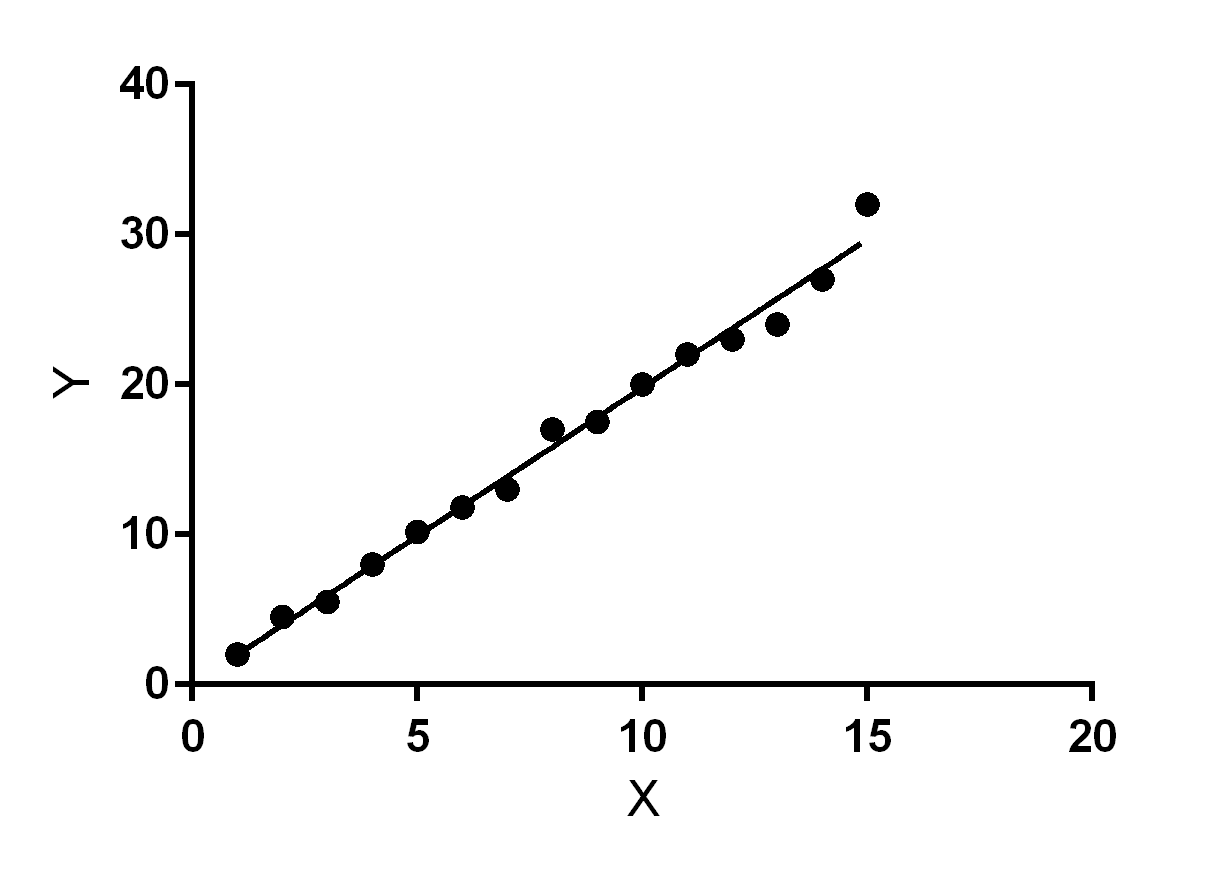
\includegraphics[scale=0.7]{Methods/Linear_regression.png}
      \end{center}
      \caption{Example linear regression}
      \label{fig:linear_regression}
  \end{figure}

  \par The way the independent variables are chosen is usually done by measuring the correlation coefficients between available features in a
  dataset and the target feature and then selecting the features having a high correlation coefficient. Depending on the problem setting, other features can be also considered 
  based on domain knowledge, especially when dealing with a mechanical system as in the case of this work. A good example of this would be the incorporation of 
  the ambient temperature measurement as an input feature---even if it does not highly correlate with the target feature---to make sure that your model generalizes when 
  trying to predict a component's temperature throughout the year, by considering the effect of seasonality 
  (temperatures are expected to be higher in summer than in winter).\\
  In this work, we selected input features based on both domain knowledge and correlation coefficients. We used Kendall's method to measure the rank correlation \cite{Kendall}.
  In contrast to Pearson's correlation coefficient, Kendall's rank correlation can capture both linear and non-linear dependency between two variables by 
  measuring the monotonic relationship. In addition to that, variables don't have to be normally distributed when using Kendall's method.

\subsection{Deep learning}
  Although multiple linear regression models are capable of fitting the data with high accuracy in many applications (e.g., \cite{Linear_Regression_Example_1}), they are,
  by definition, not capable of capturing more complex non-linear dependencies. In addition to that, linear regression may not be appropriate when there are a significant 
  number of independent variables. Deep learning may be a better approach in these situations.\\
  After obtaining better results with it (see Experiment \ref{exp:I}), we decided to train the normal behavior models
  on a feed-forward neural network (for a comprehensive review of deep learning and neural networks, see \cite{Deep_Learning}) having the architecture shown 
  in Fig. \ref{fig:MLP}.

  \begin{figure}[!htbp]
    \begin{center}
      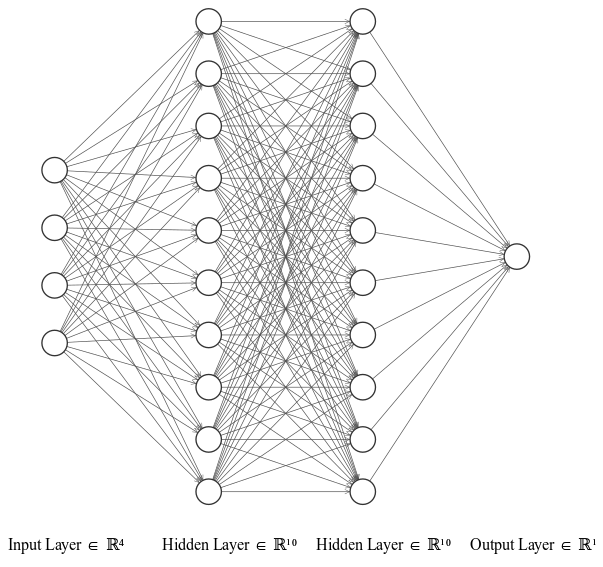
\includegraphics[scale=0.4]{Methods/MLP_cropped.png}
    \end{center}
    \caption{Architecture of normal behavior neural network model used in this work. \\
    \emph{P.S.: The input layer shape will vary based on the experiment and the number of input features.}}
    \label{fig:MLP}
  \end{figure}

  \clearpage
  
\section{Log analysis}
In this section, we will describe the different approaches we propose to utilize SCADA log messages and incorporate them into normal behavior models.
In summary, we introduce three different ways for utilizing SCADA log messages: Extracting input features for normal behavior models, Data filtering, and Visualization of warnings.
We will explain each approach in depth.

\subsection{Extracting input features}
  Most machine-learning architectures can only work with vector-shaped numerical inputs. Given that there are limited resources in the research field on how to generate 
  numerical vectors from wind turbine SCADA system logs (see chapter \ref{chap:soa}), we came up with two methods that were proven capable of not only generating input features for 
  machine-learning normal behavior models but also improving their accuracy (see chapter \ref{chap:experiments}): 1. our Novel method based on domain knowledge and 
  2. Utilizing an open-source framework for analyzing log data called LogPAI. We will discuss each method in detail.

  \subsubsection{Novel method}
    \textbf{Background:}\\
    We scanned through the different log messages available in the dataset looking for information that reflects the turbine state and might help the normal behavior model 
    fit the data more accurately. Since normal behavior models monitor the state of a component by monitoring its temperature, we narrowed the search down to operation and system logs
    that reflect events causing a change of temperature in major components. We, then, ended up with a category of logs that shows the states of internal or external ventilators
    of some components (see table \ref{tab:logs}). Being parts of the cooling systems of major components, fans or ventilators must affect the component's temperature.
    \begin{table}[H]
      \centering
      \begin{tabular}{|c|c|}
      \hline
       \textbf{Log text template} & \textbf{Log text sample}\\
       \hline
       Gen. ext. vent. \_, temp:\_\_\_\degree C & Gen. ext. vent. 2, temp:65\degree C \\
       Gen. int. vent. \_, temp:\_\_\_\degree C & Gen. int. vent. 1, temp:50\degree C \\
       HV Trafo. vent. \_, temp:\_\_\_\degree C & HV Trafo. vent. 0, temp:2\degree C \\
       Nac.vent.\_, nac/gear:\_\_\_/\_\_\_\degree C & Nac.vent.3, nac/gear:43/ 54\degree C \\
      \hline
    \end{tabular}
    \caption{Example log text templates with sample texts}
      \label{tab:logs}
    \end{table}

    Indeed, our analysis showed a clear relationship between the state of a ventilator and the temperature of its turbine component.
    As shown in Fig. \ref{fig:vent}, at low temperatures of the generator bearings, the internal ventilator will switch off. The bearings will then heat up which, in turn, causes
    the ventilator to turn on which cools the bearings down, and so on\dots

    \begin{figure}[!htbp]
      \begin{center}
        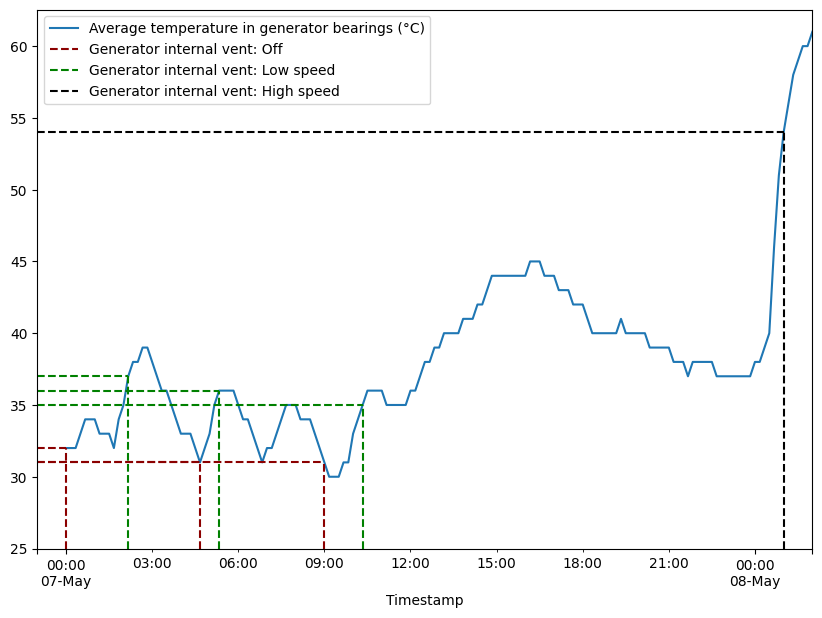
\includegraphics[scale=0.5]{Methods/Vent_Signals.png}
      \end{center}
      \caption{Generator internal vent control signals and their effect on the generator bearings temperature}
      \label{fig:vent}
    \end{figure}

    \begin{flushleft}
      \textbf{Method:}\\
      Analyzing the log texts of interest (e.g., \emph{Gen. ext. vent. 2, temp:65\degree C}), we deduce that they provide three pieces of information: 
      1. Description of the ventilator (e.g., \emph{Gen. ext. vent.}), 2. State of the ventilator (\emph{0, 1, 2 or 3}), 
      3. Temperature of the turbine component the ventilator is installed in (e.g., \emph{65\degree C}).
    \end{flushleft}
    Since the component temperature is regularly provided as a SCADA signal, we decided to focus on the other two parts of the log messages. 
    Our method simply filters log messages containing the word "vent." and creates a new feature for every ventilator (1.) found in the data having its state (2.) as a value.\\
    In contrast to the signals data fixed rate of occurrence (10 min), the generated log feature has an inconsistent frequency (the SCADA system creates a new log entry only 
    when a ventilator changes states). We join both datasets by taking the value of the last occurrence in the log feature vector within a 10-min window relative to a signal reading. 
    Gaps in the log feature columns in the resulting dataset are then filled by propagating the last valid observation forward to the next valid (a ventilator has the same state as long as it hasn't changed).\\
    Measuring the Kendall correlation factor between the generated log features and all the signals of the turbines, we found that for every temperature signal, there is at least 
    one log feature that, on average, highly correlates ($Rank>0.5$) with it.

    \begin{figure}[!htbp]
      \begin{center}
        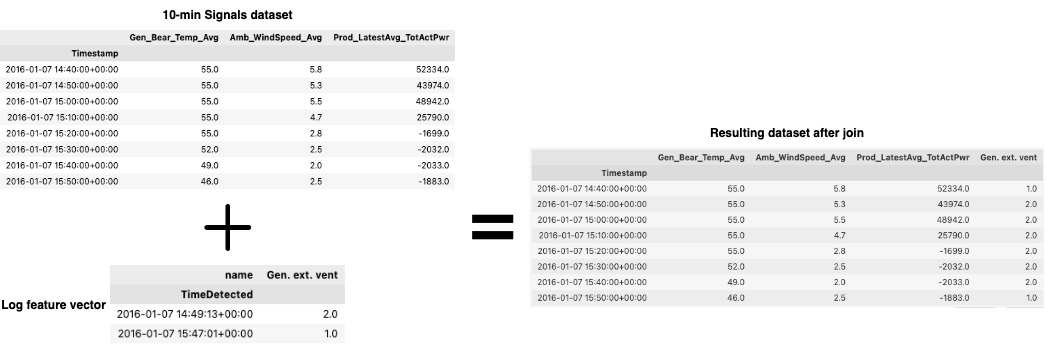
\includegraphics[scale=0.376]{Methods/Log_Merge.png}
      \end{center}
      \caption{Demonstration of the join operation between the signals 10-min dataset and a log feature vector}
      \label{fig:log-merge}
    \end{figure}
    

  \subsubsection{Utilizing LogPAI}
    LogPAI (Log Analysis and Intelligence) is a study project and open-source platform for analyzing and managing log data \cite{LogPAI}. 
    Tsinghua University researchers started the project, which focuses on developing efficient algorithms and tools for log analysis, anomaly detection, and log data visualization.
    LogPAI includes a complete suite of log analysis and processing tools such as Logparser, Loglizer, and Logreduce. 
    These applications can assist users in preprocessing and parsing raw log data, detecting anomalies and patterns, and summarizing log data concisely and understandably.
    We decided to utilize LogPAI's Logparser (\cite{Logparser_1}, \cite{Logparser_2}) and Loglizer (\cite{Loglizer}) to respectively parse and create numerical features from 
    SCADA logs in a more generic and automated way.\\
    \textbf{Preprocessing using Logparser:}\\
    From the list of parsers available in the toolkit, we decided to use Drain \cite{Drain} given that it is an online parser, which means it can process the SCADA logs 
    in real-time as they are generated. The Drain algorithm groups similar log messages together and extracts structured events from them using a 
    clustering-based approach. The research demonstrates that Drain is very good at dealing with enormous amounts of log data and extracting meaningful events from 
    noisy and diverse log data. Several phases are involved in the Drain algorithm, including log parsing, log message clustering, and event extraction. 
    Drain employs a fixed-depth tree to parse log messages into a set of log keys and their related values during the log parsing stage. The log keys 
    are unique identifiers for each type of log message, whereas the log values are the specific information connected with each log message. Drain uses a similarity measure 
    to compare the log keys and values of each log message and allocates them to the best appropriate cluster based on their similarity scores during the log message 
    clustering stage. Drain creates a template for each cluster that summarizes the relevant information contained in the log messages once the log messages have been clustered.
    Overall, the Drain algorithm makes an important contribution to log data analysis and management by providing a scalable and effective approach for extracting structured 
    events from unstructured log data.
    Applying Drain on the SCADA log data in hand by specifying its log format "\emph{<TimeDetected>,<TimeReset>,<UnitTitle>,<Content>,<UnitTitleDestination>}", we get 
    output structured log data (see Fig. \ref{fig:logparser} for an example) that the Loglizer can process to generate numerical features.

    \begin{figure}[!htbp]
      \begin{center}
        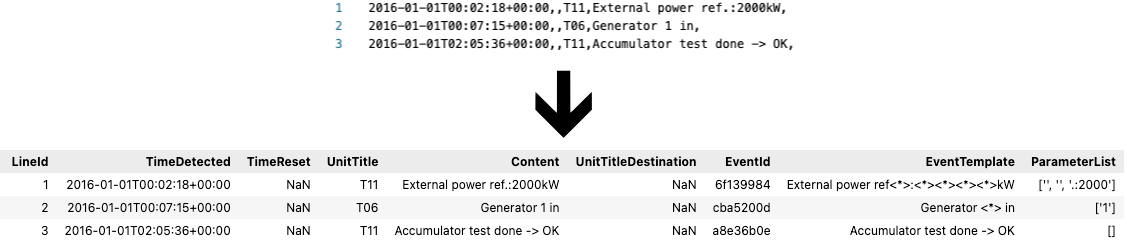
\includegraphics[scale=0.349]{Methods/Logparser.png}
      \end{center}
      \caption{Sample raw logs and their corresponding structured logs after being parsed by Drain}
      \label{fig:logparser}
    \end{figure}

    \begin{flushleft}
      \textbf{Creating numerical features using Loglizer}:\\
      Loglizer's \emph{Feature Extraction} component supports various feature extraction techniques, such as Bag-of-Words, TF-IDF, and Word2Vec, 
      to capture the essential information contained in log data. We utilized the Loglizer feature extractor, using TF-IDF \cite{TF-IDF} for term weighting, to generate numerical 
      features from the parsed logs' \emph{Event IDs}. 
    \end{flushleft}

\subsection{Data filtering}
  TODO:
  Stoppages (log as filter)

\subsection{Visualization of warnings}
  TODO:
  Easy: look for any warning/alarm message (having the word "hot" or "high temperature") related to the target component (having the name of the component in the message) 
  and append to the anomaly on the operation dashboard

  \clearpage

\section{Anomaly detection}
  TODO:
  Define anomalies (what is an anomaly in general?).\\
  Discuss anomaly detection methods used in other papers\\
  Argue why there's no standard way of defining/measuring an anomaly\\
  Describe the way our anomaly detection works.

\subsection{Alarms}
  TODO:
  Discuss the difference between Anomaly and alarm and why we wanna limit the number of alarms being sent to operators (false alarms are costly!)

\section{Summary}
TODO:
PUSH TO THE TOP//
Diagram of all methods put together: ML model + log feature + Anomaly detection + Alarms,...
\chapter{Experiments}
\label{chap:experiments}
In this chapter, we describe a set of experiments we ran to quantitatively and qualitatively measure the effect of incorporating the log embeddings introduced into normal behavior models
when applied to both \emph{healthy} and \emph{faulty} turbines. For a normal behavior model monitoring a component of a turbine, we considered this turbine \emph{faulty} if 
a failure was reported, in the failures dataset, related to this specific component of this turbine. It is considered \emph{healthy} if no failures, relating to this turbine's component,
were reported.\\
To compare different models in an identical setup, we use the following metrics:
\begin{bulletList}
    \item \textbf{Root Mean Squared Error ($RMSE$)}: It is a commonly used metric to evaluate the performance of a predictive model or an estimator.
    The $RMSE$ is calculated as the square root of the mean of the squared differences between the predicted ($y_{predicted}$) and actual values ($y_{actual}$), or as follows:
    \begin{equation}
        RMSE = \sqrt{\frac{1}{n} * \sum_{i}^{n} (y_{predicted}^i - y_{actual}^i)^2}
    \end{equation}
    where $n$ is the number of data points in a dataset. The RMSE is expressed in the same units as the original data. 
    As a rule of thumb: The lower the RMSE, the better the model fits the data.
    \item \textbf{Numbers of anomalies and alarms detected during a given period}: We use these numbers to measure the capability of a model to detect/predict a failure. 
    The number of anomalies detected reflects the total number of anomalous data points, whereas the number of alarms detected counts only the number of operation days of a turbine 
    where the system notified the operator of a potential failure by sending an alarm (if the number of anomalies detected in a day exceeds a certain threshold, 
    as explained in \ref{subsub:anvsal}). When compared to another model, we consider a model more \emph{capable} of predicting failures if it 
    detects more anomalies and/or sends more alarms during the time of abnormal operation of a faulty turbine given that it reported no anomalies or alarms during the normal operation 
    of the same turbine. In other words, we compare these metrics between models when applied to the test data of a faulty turbine, assuming that the data used to train these models 
    was collected from the turbine in a period when it was operating in a healthy state; hence no anomalies should be detected in this period.
    \item \textbf{Timestamps of the first anomaly detected and alarm sent}: Used to compare the capability of different models to early-detect failures, when applied to a faulty turbine. The earlier
    the first anomaly is detected or the first alarm is sent the better.
\end{bulletList}
All the condition monitoring normal behavior models used in our experiments were trained to monitor the generator bearings of a turbine (i.e., having the average temperature in the generator bearings 
as a target), whereas the power curve normal behavior models monitor the average power production of a turbine according to the grid (in kW). The input features used are listed in \ref{sub:featselect}.

%Experiment I
\section{Benchmark NBM architecture}
\label{exp:I}

In the early stages of this work, we trained linear regression models due to their lightweight and low computational power needed. Knowing that they are incapable of capturing non-linear
relationships in the data, we assumed that the linear regression models would be outperformed by feed-forward neural networks when it comes down to fitting the 
signals data of a healthy turbine. To test this hypothesis and select a specific architecture to be used as a benchmark NBM model in other experiments, we did this simple experiment 
to compare the $RMSE$ scores of both models.\\
This experiment was conducted on a healthy turbine (Turbine 01). Both models were trained on signals data collected between 01/09/2016 and 30/08/2017 and tested on data collected between
01/09/2017 and 31/12/2017.\\
As shown in Table \ref{tab:Experiment I results}, the feed-forward network outperformed the linear regression model---as expected---and was used as a baseline in all the other experiments.
\begin{table}[H]
        \centering
    \begin{tabular}{|c|c|c|}
    \hline
         \textbf{Metric} & \textbf{Linear regression} & \textbf{Feed-forward network}\\
         \hline
         Training RMSE & 5.29 & 4.86\\
         \hline
         Testing RMSE & 5.80 & 5.78 \\
    \hline
    \end{tabular}
    \caption{Experiment I results: RMSEs measured and used to compare the benchmark models}
        \label{tab:Experiment I results}
\end{table}

%Experiment II

\section{Effect of incorporating log embeddings into NBM for condition monitoring when applied to a healthy turbine (T01)}
\subsection{Setup}
This experiment aims to quantitatively and qualitatively measure 
the effect of incorporating SCADA-log-based embeddings into the baseline normal behavior model when applied to a healthy turbine.
(see method \ref{sub:dk_method} and \ref{subsub:Loglizer})\\
We ran this experiment three times: one time using the baseline normal behavior model (i.e., using only SCADA signals as input features), 
repeated once after adding the log embeddings generated based on domain knowledge as input features (denoted as \emph{Model-DK}), and 
another time after incorporating LogPAI-generated log embeddings (denoted as \emph{Model-PAI}).
The models were trained on data collected between 01/09/2016 and 30/08/2017 and tested on data collected between
01/09/2017 and 31/12/2017.\\
As shown in Table \ref{tab:expII:domain-knowledge-feats}, all log embeddings generated based on domain knowledge highly correlate with the target feature 
and were hence used as input features in \emph{Model-DK} in addition to the selected SCADA signals.
As for the log embeddings generated using LogPAI, only a few features were found to relatively highly correlate (correlation factor greater than 0.3 or less than -0.3) 
with the target feature (see Table \ref{tab:expII:logpai-feats}) and were selected, in addition to the selected SCADA signals, as input features in \emph{Model-PAI}.
\begin{table}[H]
    \parbox{.45\linewidth}{
    \centering
    \begin{tabular}{|c|c|}
        \hline
        Feature & Correlation\\
        \hline
        \multicolumn{1}{|m{0.25\textwidth}|}{Generator external ventilator} & 0.713057\\
        \hline
        \multicolumn{1}{|m{0.25\textwidth}|}{Generator internal ventilator} & 0.730726\\
        \hline
        \multicolumn{1}{|m{0.25\textwidth}|}{High-voltage transformer ventilator} & 0.513700\\
        \hline
        \multicolumn{1}{|m{0.25\textwidth}|}{Nacelle ventilator} & 0.514112\\
        \hline
    \end{tabular}
    \caption{Measures of Kendall's correlation between the domain knowledge-based log embeddings and the target feature in Turbine 01}
    \label{tab:expII:domain-knowledge-feats}
    }
    \hfill
    \parbox{.45\linewidth}{
    \centering
    \begin{tabular}{|c|c|}
        \hline
        Feature & Correlation\\
        \hline
        \multicolumn{1}{|m{0.25\textwidth}|}{\hl{LogPAI Feature 1}} & \hl{-0.335313}\\
        \hline
        \multicolumn{1}{|m{0.25\textwidth}|}{\hl{LogPAI Feature 2}} & \hl{-0.320031}\\
        \hline
        \multicolumn{1}{|m{0.25\textwidth}|}{LogPAI Feature 3} & 0.015902\\
        \hline
        \multicolumn{1}{|m{0.25\textwidth}|}{LogPAI Feature 4} & -0.220749\\
        \hline
        \multicolumn{1}{|m{0.25\textwidth}|}{LogPAI Feature 5} & 0.083943\\
        \hline
        \multicolumn{1}{|m{0.25\textwidth}|}{\hl{LogPAI Feature 6}} & \hl{-0.303429}\\
        \hline
        \multicolumn{1}{|m{0.25\textwidth}|}{LogPAI Feature 7} & 0.191848\\
        \hline
        \multicolumn{1}{|m{0.25\textwidth}|}{LogPAI Feature 8} & -0.045460\\
        \hline
        \multicolumn{1}{|m{0.25\textwidth}|}{LogPAI Feature 9} & -0.077507\\
        \hline
        \multicolumn{1}{|m{0.25\textwidth}|}{LogPAI Feature 10} & -0.157537\\
        \hline
        \multicolumn{1}{|m{0.25\textwidth}|}{LogPAI Feature 11} & -0.102636\\
        \hline
        \multicolumn{1}{|m{0.25\textwidth}|}{LogPAI Feature 12} & 0.018344\\
        \hline
        \multicolumn{1}{|m{0.25\textwidth}|}{LogPAI Feature 13} & 0.244219\\
        \hline
        \multicolumn{1}{|m{0.25\textwidth}|}{LogPAI Feature 14} & -0.129601\\
        \hline
        \multicolumn{1}{|m{0.25\textwidth}|}{\hl{LogPAI Feature 15}} & \hl{0.361669}\\
        \hline
        \multicolumn{1}{|m{0.25\textwidth}|}{LogPAI Feature 16} & -0.010470\\
        \hline
    \end{tabular}
    \caption{Measures of Kendall's correlation between the log embeddings generated based on the event IDs using the LogPAI framework and the target feature in Turbine 01. Selected features are highlighted.}
    \label{tab:expII:logpai-feats}
    }
    \end{table}

At this stage, the main goal is to test whether those highly-correlating features would improve the baseline model, or, 
they provide redundant information that could be indirectly deduced from the signal features.

\subsection{Results}
\subsubsection{Performance}
As reported in Table \ref{tab:Experiment II results}, the incorporated log embeddings, both in \emph{Model-DK} and \emph{Model-PAI}, improved the RMSE scores of the models. 
This shows that those features provided additional information to the model that wasn't available in the selected SCADA signals, which shows that our proposed methods 
were indeed capable of retrieving valuable information from the SCADA logs.

\begin{table}[H]
    \centering
\begin{tabular}{|c|c|c|c|}
\hline
     \textbf{Metric} & \textbf{\emph{Baseline}} & \textbf{\emph{Model-DK}} & \textbf{\emph{Model-PAI}}\\
     \hline
     Training RMSE & 4.864 & 4.087 & 4.617\\
     \hline
     Testing RMSE & 5.784 & 5.195 & 5.607\\
\hline
\end{tabular}
\caption{Experiment results: RMSEs measured and used to compare between the \emph{Baseline} model, \emph{Model-DK}, and \emph{Model-PAI} when applied to Turbine 01}
    \label{tab:Experiment II results}
\end{table}

\subsubsection{Anomaly detection}
Applying the models to the testing dataset, 12, 15, and 8 data points were labeled anomalous by the \emph{Baseline} model,
\emph{Model-DK}, and \emph{Model-PAI}, respectively. Those anomalous data points were spread over 4 days for all three models. 
Whether to consider these data points as false positives or not is 
arguable. One could consider them as false positives based on the premise that the turbine was operating in a healthy state.
In this case, \emph{Model-PAI} would be ranked highest in terms of anomaly detection. However, these data points could indeed
be anomalous and be signaling a fault that might happen in the future. Here, \emph{Model-DK} would show a higher sensitivity 
to anomalous data points. \\
Given that the dataset provided doesn't include data from the following years (2018+), 
we weren't able to test the different possibilities and will leave the interpretation open to the reader.\\

No alarms were reported in all three models. This result shows that none of the anomalies detected was considered 
critical enough for the operator to be notified, which aligns with the assumption that the turbine is healthy.
A summary of the discussed results is shown in Table \ref{tab:summary_expII}.

\begin{table}[H]
    \centering
    \begin{tabular}{|c|c|c|c|}
        \hline
            \textbf{Metric} & \textbf{\emph{Baseline}} & \textbf{\emph{Model-DK}} & \textbf{\emph{Model-PAI}}\\
            \hline
            \#Anomalous data points & 12 & 15 & 8\\
            \hline
            ..firstly detected on & 04/12/2017 & 15/11/2017 & 04/12/2017\\
            \hline
            ..lastly detected on & 27/12/2017 & 27/12/2017 & 27/12/2017\\
            \hline
            \#Anomalous days & 4 & 4 & 4\\
            \hline
            ..of which warning logs were found & 0 & 0 & 0\\
            \hline
            \#Alarms sent & 0 & 0 & 0\\
        \hline
    \end{tabular}
    \caption{Summary of experiment results}
    \label{tab:summary_expII}
\end{table}






%Experiment III

\section{Effect of incorporating log embeddings into NBM for condition monitoring when applied to a faulty turbine (T09)}
\subsection{Setup}
This experiment aims to quantitatively and qualitatively measure 
the effect of incorporating SCADA-log-based embeddings into the baseline normal behavior model when applied to a faulty turbine 
(see method \ref{sub:dk_method}, \ref{subsub:vis_warnings}, and \ref{subsub:Loglizer}).\\
For this turbine (T09), several failures relating to the generator bearings were reported starting on 07/06/2016 and ending on 17/10/2016
by replacing the generator bearings (see Table \ref{tab:failures}). In this case, not only do we want to measure the performance of our models fitting the data 
during the presumably healthy (training) period, but also we want to test their capability of detecting the recorded failures early and notifying the operator 
in cases of major anomalies in the operation of the turbine's component.\\
We ran this experiment three times: one time using the baseline normal behavior model (i.e., using only SCADA signals as input features), 
repeated once after adding the log embeddings generated based on domain knowledge as input features (denoted as \emph{Model-DK}), and 
another time after incorporating LogPAI-generated log embeddings (denoted as \emph{Model-PAI}).
The models were trained on data collected between 01/01/2016 and 15/02/2016 and tested on data collected between
16/02/2016 and 18/10/2016. Due to the limits of the dataset at hand, only two and a half months of data could be used to train the models since, 
according to our analysis, this is the period where the turbine was assumably still operating in healthy conditions.
Due to the shortage in the training dataset, some features in the testing dataset were found to be out-of-distribution (see Fig. \ref{fig:Boxplot_T09}). 
This fact made the interpretation of the results a bit more challenging, it, however, helped test the robustness of the 
different models' architectures.

\begin{figure}[h]
    \begin{center}
      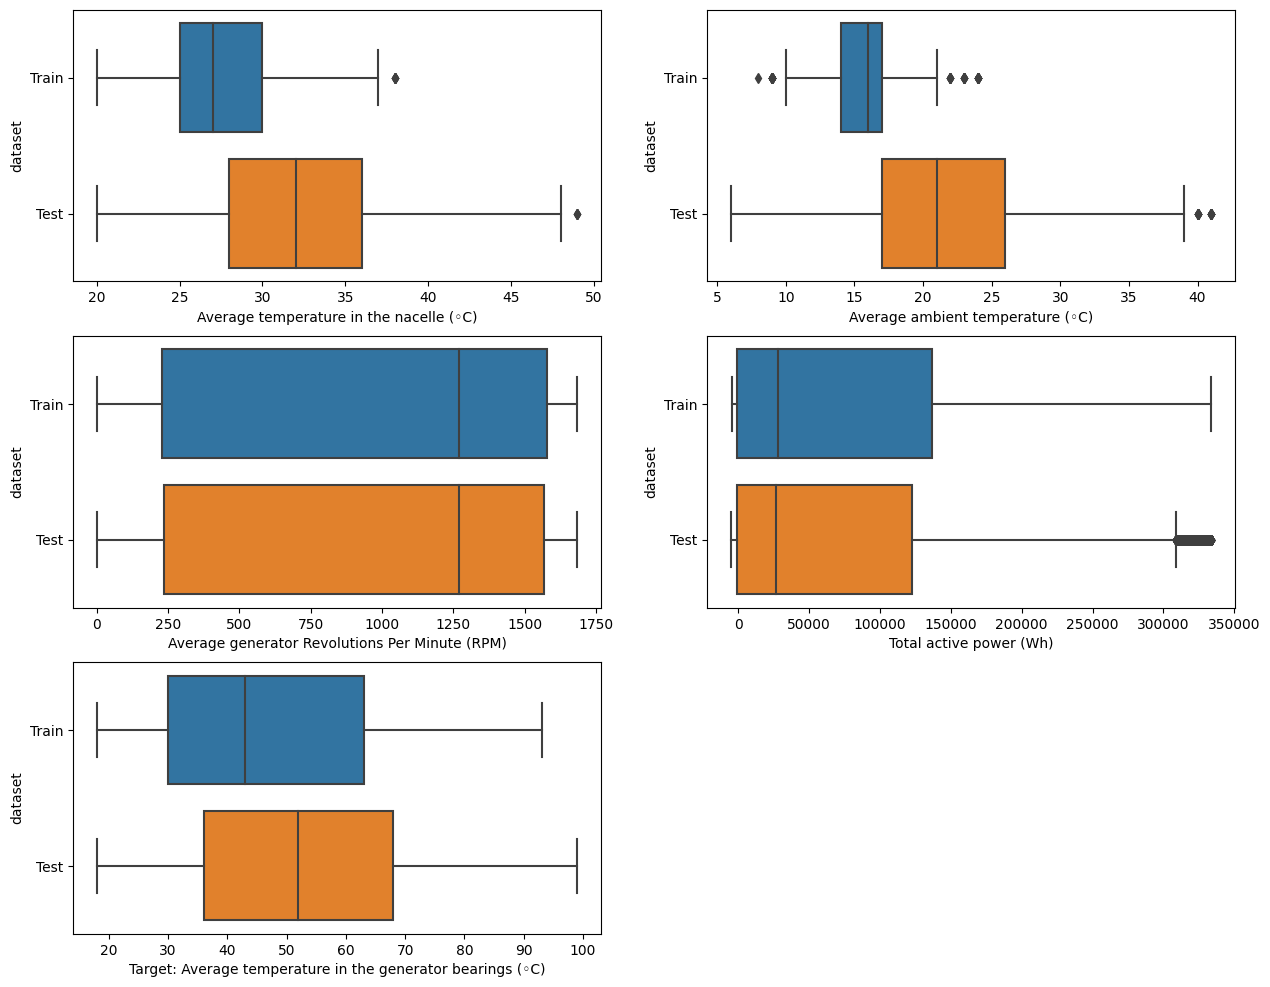
\includegraphics[scale=0.43]{Experiments/Boxplot_T09.png}
    \end{center}
    \caption{Boxplots showing the distribution of signals collected from Turbine 09 sensors used to train and test the models}
    \label{fig:Boxplot_T09}
  \end{figure}

As shown in Table \ref{tab:expIII:domain-knowledge-feats}, all log embeddings generated based on domain knowledge highly correlate with the target feature 
and were hence used as input features in \emph{Model-DK} in addition to the selected SCADA signals.
As for the log embeddings generated using LogPAI, only two features were found to relatively highly correlate (correlation factor greater than 0.3 or less than -0.3) 
with the target feature (see Table \ref{tab:expIII:logpai-feats}) and were selected, in addition to the selected SCADA signals, as input features in \emph{Model-PAI}.
\begin{table}[h]
    \parbox{.45\linewidth}{
    \centering
    \begin{tabular}{|c|c|}
        \hline
        Feature & Correlation\\
        \hline
        \multicolumn{1}{|m{0.25\textwidth}|}{Generator external ventilator} & 0.505995\\
        \hline
        \multicolumn{1}{|m{0.25\textwidth}|}{Generator internal ventilator} & 0.656839\\
        \hline
        \multicolumn{1}{|m{0.25\textwidth}|}{High-voltage transformer ventilator} & 0.500316\\
        \hline
        \multicolumn{1}{|m{0.25\textwidth}|}{Nacelle ventilator} & 0.480353\\
        \hline
    \end{tabular}
    \caption{Measures of Kendall's correlation between the domain knowledge-based log embeddings and the target feature in Turbine 09}
    \label{tab:expIII:domain-knowledge-feats}
    }
    \hfill
    \parbox{.45\linewidth}{
    \centering
    \begin{tabular}{|c|c|}
        \hline
        Feature & Correlation\\
        \hline
        \multicolumn{1}{|m{0.25\textwidth}|}{LogPAI Feature 1} & -0.279547\\
        \hline
        \multicolumn{1}{|m{0.25\textwidth}|}{LogPAI Feature 2} & 0.026935\\
        \hline
        \multicolumn{1}{|m{0.25\textwidth}|}{\hl{LogPAI Feature 3}} & \hl{-0.320831}\\
        \hline
        \multicolumn{1}{|m{0.25\textwidth}|}{LogPAI Feature 4} & 0.019996\\
        \hline
        \multicolumn{1}{|m{0.25\textwidth}|}{LogPAI Feature 5} & -0.296431\\
        \hline
        \multicolumn{1}{|m{0.25\textwidth}|}{LogPAI Feature 6} & 0.018961\\
        \hline
        \multicolumn{1}{|m{0.25\textwidth}|}{LogPAI Feature 7} & 0.231462\\
        \hline
        \multicolumn{1}{|m{0.25\textwidth}|}{LogPAI Feature 8} & -0.214312\\
        \hline
        \multicolumn{1}{|m{0.25\textwidth}|}{LogPAI Feature 9} & 0.172929\\
        \hline
        \multicolumn{1}{|m{0.25\textwidth}|}{\hl{LogPAI Feature 10}} & \hl{0.324340}\\
        \hline
        \multicolumn{1}{|m{0.25\textwidth}|}{LogPAI Feature 11} & -0.131364\\
        \hline
        \multicolumn{1}{|m{0.25\textwidth}|}{LogPAI Feature 12} & -0.011957\\
        \hline
        \multicolumn{1}{|m{0.25\textwidth}|}{LogPAI Feature 13} & -0.080340\\
        \hline
        \multicolumn{1}{|m{0.25\textwidth}|}{LogPAI Feature 14} & -0.158273\\
        \hline
        \multicolumn{1}{|m{0.25\textwidth}|}{LogPAI Feature 15}& -0.126988\\
        \hline
        \multicolumn{1}{|m{0.25\textwidth}|}{LogPAI Feature 16} & -0.074183\\
        \hline
    \end{tabular}
    \caption{Measures of Kendall's correlation between the log embeddings generated based on the event IDs using the LogPAI framework and the target feature in Turbine 09. Selected features are highlighted.}
    \label{tab:expIII:logpai-feats}
    }
    \end{table}

At this stage, the main goal is to test whether the generated log embeddings would also improve the performance of the baseline model when applied to a 
faulty turbine. In addition to that, we want to test the effect of these features on improving the model's capability of failure early detection.
For that, we start by measuring the RMSE scores to compare the models' performances and then analyze the anomalies detected in the testing period 
and the yielded alarms.

\subsection{Results}
\subsubsection{Performance}
Again, it was shown that the incorporated log embeddings, both in \emph{Model-DK}, and \emph{Model-PAI}, improved the RMSE scores of the models (see Table \ref{tab:Experiment III results}). 

\begin{table}[H]
    \centering
\begin{tabular}{|c|c|c|c|}
\hline
     \textbf{Metric} & \textbf{\emph{Baseline}} & \textbf{\emph{Model-DK}} & \textbf{\emph{Model-PAI}}\\
     \hline
     Training RMSE & 8.562 & 8.081 & 8.386\\
     \hline
     Testing RMSE & 9.084 & 8.936 & 9.029\\
\hline
\end{tabular}
\caption{Experiment results: RMSEs measured and used to compare between the \emph{Baseline} model, \emph{Model-DK}, and \emph{Model-PAI} when applied to Turbine 09}
    \label{tab:Experiment III results}
\end{table}

\subsubsection{Anomaly \& Early fault detection}
In total, 48, 217, and 236 anomalies were reported by the \emph{Baseline} model, \emph{Model-DK}, and \emph{Model-PAI}, respectively.
Those anomalous data points were spread over 29 days for the \emph{Baseline} model, 42 days for \emph{Model-DK}, and 53 days for \emph{Model-PAI}.
From these anomalous days, relevant alarm and warning logs were found (see \ref{subsub:vis_warnings} on how these logs are retrieved) on 18 days for both \emph{Model-DK} and \emph{Model-PAI} and only 14 days for the \emph{Baseline} model.
In addition to that, both \emph{Model-DK} and \emph{Model-PAI} detected the first anomaly one day earlier than the \emph{Baseline} model (16/02/2016 versus 17/02/2016).

This result only shows the major effect of the log embeddings---whether the ones generated by applying domain knowledge or using LogPAI---on the behavior of 
the model during unhealthy conditions of the turbine. The way we interpret this result is as follows: By adding supplementary information regarding the turbine's control signals
found in the SCADA log, the model could provide a better simulation of the turbine in healthy conditions and, hence, detect abnormalities more easily
during unhealthy states of operation.\\
Using the method described in \ref{subsub:anvsal}, only \emph{Model-DK} sent alarms with a total of six alarms starting on 19/02/2016 and ending on 23/08/2016.
This is due to the fact that the peak number of anomalies detected per day was significantly higher for \emph{Model-DK} (between 13 and 28) 
compared to \emph{Model-PAI} (12) and the \emph{Baseline} model (3 only). 
On one hand, we believe this result is due to the limited sample size used to train the model. 
However, on the other hand, it shows the higher robustness of \emph{Model-DK}: the limited training dataset was enough for the model 
to report higher numbers of anomalies detected per day during the validation period, high enough for it to trigger several alarms.\\
A summary of the discussed results is shown in Table \ref{tab:summary_expIII}.

\begin{table}[H]
    \centering
    \begin{tabular}{|c|c|c|c|}
        \hline
            \textbf{Metric} & \textbf{\emph{Baseline}} & \textbf{\emph{Model-DK}} & \textbf{\emph{Model-PAI}}\\
            \hline
            \#Anomalous data points & 48 & 217 & 236\\
            \hline
            ..firstly detected on & 17/02/2016 & 16/02/2016 & 16/02/2016\\
            \hline
            ..lastly detected on & 29/09/2016 & 06/10/2016 & 11/10/2016\\
            \hline
            \#Anomalous days & 29 & 42 & 53\\
            \hline
            ..of which warning logs were found & 14 & 18 & 18\\
            \hline
            \#Alarms sent & 0 & 6 & 0\\
            \hline
            ..firstly on & \- & 19/02/2016 & \-\\
            \hline
            ..lastly on & \- & 23/08/2016 & \-\\
        \hline
    \end{tabular}
    \caption{Summary of experiment results: Anomaly and early detection of faulty generator bearings which were replaced on 17/10/2016}
    \label{tab:summary_expIII}
\end{table}

\section{Effect of log-based data filtering on NBM for power curve modeling}
    \label{sec:Experiment IV}
    \subsection{Setup}
    The main goal of this experiment is to test the effectiveness of method \ref{subsub:PC} in improving normal behavior models 
    having power production as the target, also known as power curve models. To do so, we trained a normal behavior model on 
    data collected from Turbine 01 sensors between September 2016 and August 2017 and tested it on data collected between September 2017 
    and December 2017. We used only the ambient wind speed (m/s) and ambient temperature (\degree C) signals as input features 
    and the average power production according to the grid (kW) as the target feature.\\
    We trained three different models having the same architecture but using different datasets: 
    Using all the raw signals collected; denoted as \emph{Baseline}, 
    using raw signals when the turbine was spinning only (i.e., rotor speed greater than zero); denoted as \emph{Model-Spin},
    and using raw signals when the turbine was operating in a "Run" state only based on the SCADA log; denoted as \emph{Model-Run}.\\

    Figure \ref{fig:labels} shows how the data points are labeled based on the filters explained. One could see that \emph{Model-Spin} 
    doesn't consider all data points where the turbine isn't spinning (red and yellow points) including when it's in a "Run" state
    but the wind speed hasn't reached the cut-in speed yet (yellow points). Although \emph{Model-Run} will also not consider some of the data points
    where the turbine is not spinning (red points), it will still consider the yellow points. In addition to that, it will exclude data points 
    where the turbine is in a "Stop" state but still spinning (most probably still in the transition phase after gradually applying the brakes).
    The \emph{Baseline} is simply trained on all the data points.

    \begin{figure}[H]
        \begin{center}
          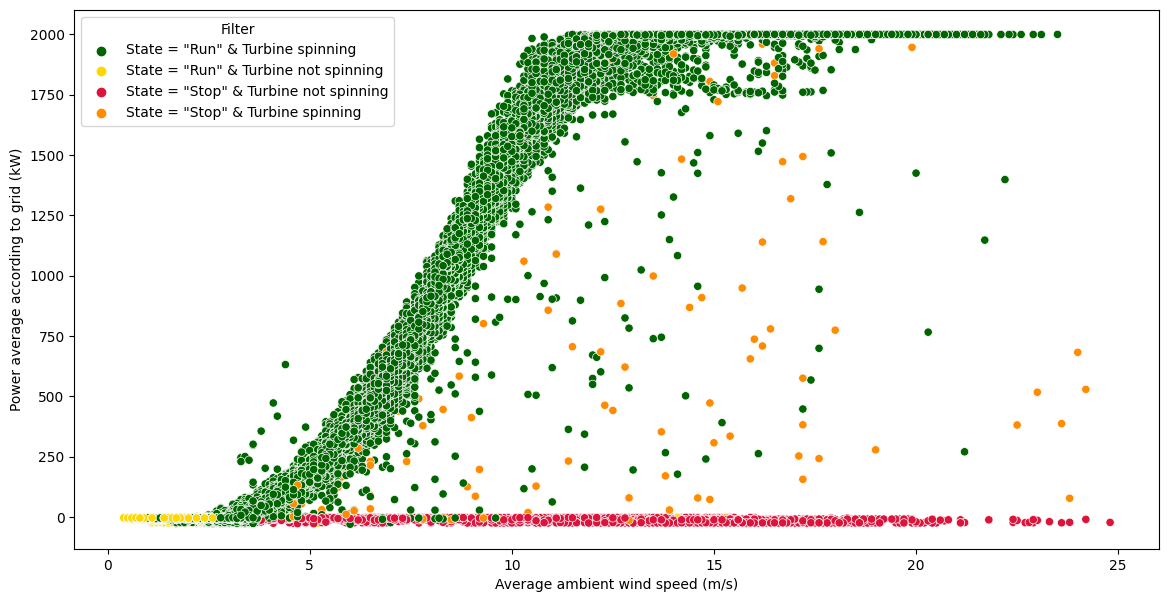
\includegraphics[scale=0.45]{Experiments/labels.png}
        \end{center}
        \caption{Turbine 01 power curve: Data points labeled based on different filters}
        \label{fig:labels}
      \end{figure}
    
      \subsection{Results}
      Here, we simply compared the models' performances by measuring their RMSE scores. Comparing the models' anomaly detection 
      and performance evaluation capabilities wasn't in the scope of this work, as we mainly focused on analyzing the generator-related condition 
      monitoring models. We did however reach these results while analyzing different strategies to utilize the SCADA logs in the 
      context of SCADA-based condition monitoring and decided they were worth documenting.\\

      Table \ref{tab:Experiment IV results} shows the measured RMSE scores of the three models. As shown, filtering the data improved
      the model's performance drastically. The filtering based on the turbine's state retrieved from the SCADA logs (\emph{Model-Run}) 
      yielded the best results in this setting. This shows that the generated labels provide valuable insights into the turbine's state 
      and can be used instead of a simple filter by the rotor's speed, especially if the latter isn't available as a SCADA signal for a given turbine.
      Figure \ref{fig:3pcs} also shows the better power curve fit both \emph{Model-Spin} and \emph{Model-Run} have compared to the \emph{Baseline} model 
      when applied to the testing dataset.

      \begin{table}[h]
        \centering
    \begin{tabular}{|c|c|c|c|}
    \hline
         \textbf{Metric} & \textbf{\emph{Baseline}} & \textbf{\emph{Model-Spin}} & \textbf{\emph{Model-Run}}\\
         \hline
         Training RMSE & 179.200 & 61.707 & 51.309\\
         \hline
         Testing RMSE & 139.972 & 59.988 & 50.251\\
    \hline
    \end{tabular}
    \caption{Experiment results: RMSEs measured and used to compare between the \emph{Baseline} model, \emph{Model-Spin} and \emph{Model-Run} when applied to Turbine 01}
        \label{tab:Experiment IV results}
    \end{table}

    \begin{figure}[h]
        \begin{center}
          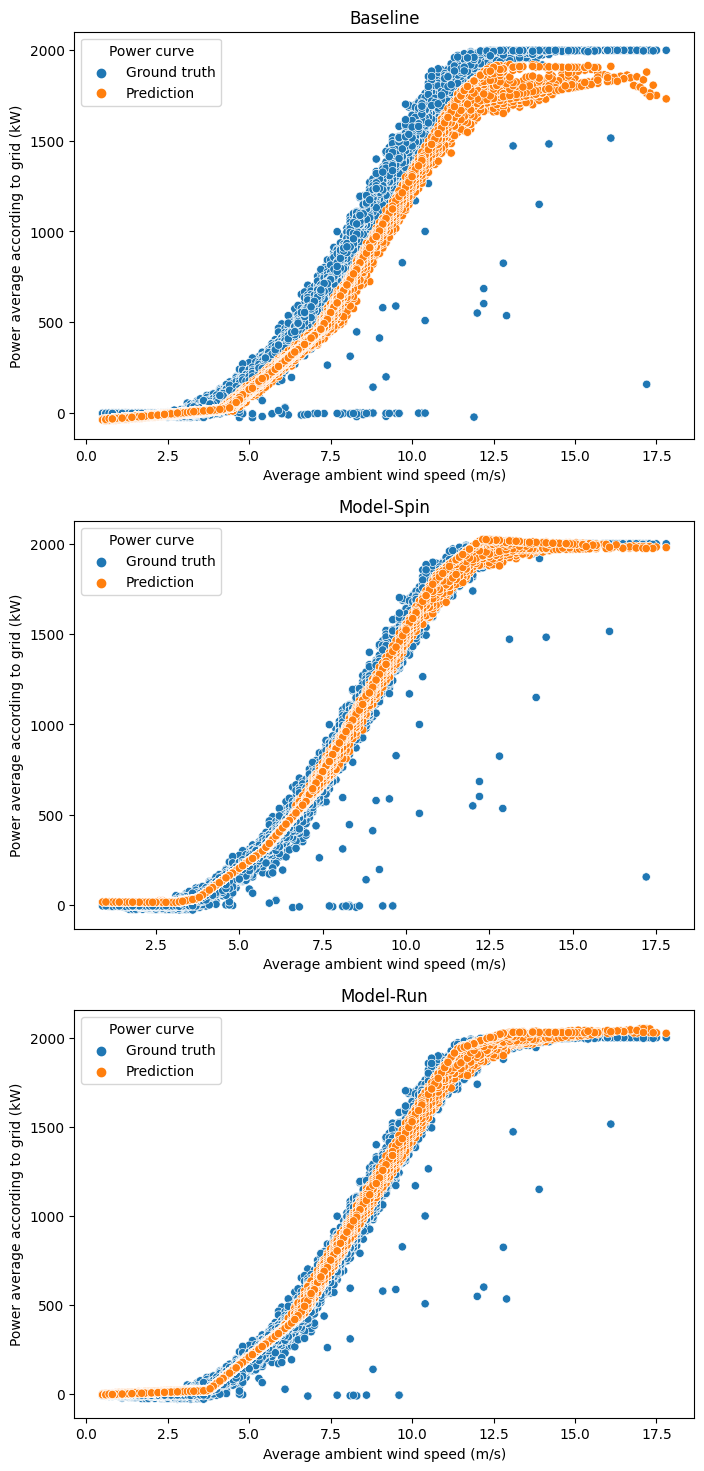
\includegraphics[scale=0.5]{Experiments/3pcs.png}
        \end{center}
        \caption{True versus predicted power curves of the \emph{Baseline} model, \emph{Model-Spin}, and \emph{Model-Run}, respectively, 
        when applied to the testing dataset of Turbine 01}
        \label{fig:3pcs}
      \end{figure}
    


\chapter{Conclusions and Future Works}
\label{chap:conclusions}

\section{Conclusions}

\section{Future Works}
\label{sec:future_works}

\appendix

\chapter{Wind Turbine Characteristics}
\label{chap:appendix1}

Here, we list the characteristics of the turbines whose data was used in our experiments.
The following table shows the technical characteristics of these Vestas turbines:

\begin{table}[H]
    \centering
    \begin{tabular}{|c|c|c|c|}
    \hline
    \multirow{5}{*}{\rotatebox[origin=c]{90}{Power}} & Rated power (kW) & 2,000 \\
    & Cut-in wind speed (m/s) & 4 \\
    & Rated wind speed (m/s) & 12  \\
    & Cut-out wind speed (m/s) & 25 \\
    & Wind class (IEC) & IEC II (7.5 - 8.5 m/s) \\
    \hline
    \multirow{7}{*}{\rotatebox[origin=c]{90}{Rotor}} & Diameter (m) & 90 \\
    & Swept area (m\textsuperscript{2}) & 6,362 \\
    & Number of blades & 3  \\
    & Rotor speed, max (rpm) & 14.9 \\
    & Tip speed (m/s) & 70 \\
    & Power density 1 (W/m\textsuperscript{2}) & 314.4 \\
    & Power density 2 (m\textsuperscript{2}/kW) & 3.2 \\
    \hline
    \multirow{4}{*}{\rotatebox[origin=c]{90}{Gearbox}} & & \\
    & Type & Planetary/spur \\
    & Stages (m/s) & 3 \\
    & & \\
    \hline
    \multirow{4}{*}{\rotatebox[origin=c]{90}{Generator}} & Type & Asynchronous \\
    & Speed, max (rpm) & 2,016 \\
    & Voltage (V) & 690  \\
    & Grid frequency (Hz) & 50 \\
    \hline
    \multirow{4}{*}{\rotatebox[origin=c]{90}{Tower}} & Hub height (m) & 80 \\
    & Type & Steel tube \\
    & Shape & Conical  \\
    & Corrosion protection & Painted \\
    \hline
    \end{tabular}
    \caption{Wind turbine characteristics}
    \label{tab:characteristics}
\end{table}

The following graph demonstrates the turbines' power curve provided by the manufacturer:

\begin{figure}[H]
    \begin{center}
      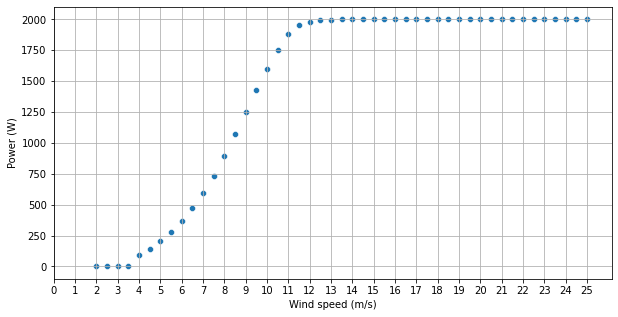
\includegraphics[scale=0.6]{Appendix1/Power_curve.png}
    \end{center}
    \caption{Power curve of the Vestas turbines at an air density of 1.225 kg/m\textsuperscript{3}}
  \end{figure}
\chapter{Recorded Failures}
\label{chap:appendix2}
Here, we show the full list of failures detected in all five turbines and recorded by the technicians or the service company.
These failures were found and documented upon on-site inspections and were used to validate the capability of the normal behavior models to 
predict them early (enough) before actually occurring. Table \ref{tab:failures} shows the full list of failures.

\begin{table}[H]
    \centering
    \begin{tabular}{|c|c|c|c|}
    \hline
    \textbf{Turbine} & \textbf{Component} & \textbf{Recorded at} & \textbf{Technician Remarks} \\
    \hline
    \multirow{2}{*}{01} & Gearbox & 2016-07-18 02:10:00 & Gearbox pump damaged \\
    & Transformer & 2017-08-11 13:14:00 & Transformer fan damaged \\
    \hline
    \multirow{9}{*}{06} & Hydraulic group & 2016-04-04 18:53:00 & Error in pitch regulation \\
    & Generator & 2016-07-11 19:48:00 & Generator replaced \\
    & Generator & 2016-07-24 17:01:00 & Generator temperature sensor failure \\
    & Generator & 2016-09-04 08:08:00 & High temperature generator error \\
    & Generator & 2016-10-02 17:08:00 & Refrigeration system and \\
    & & & temperature sensors in generator replaced \\
    & Generator & 2016-10-27 16:26:00 & Generator replaced \\
    & Hydraulic group & 2017-08-19 09:47:00 & Oil leakage in Hub \\
    & Gearbox & 2017-10-17 08:38:00 & Gearbox bearings damaged \\
    \hline
    \multirow{9}{*}{07} & Generator bearings & 2016-04-30 12:40:00 & High temperature in generator bearing \\
    & & & (replaced sensor) \\
    & Transformer & 2016-07-10 03:46:00 & High temperature transformer \\
    & Transformer & 2016-08-23 02:21:00 & High temperature transformer. \\
    & & & Transformer refrigeration repaired \\
    & Hydraulic group & 2017-06-17 11:35:00 & Oil leakage in Hub \\
    & Generator bearings & 2017-08-20 06:08:00 & Generator bearings damaged \\
    & Generator & 2017-08-21 14:47:00 & Generator damaged \\
    & Hydraulic group & 2017-10-19 10:11:00 & Oil leakage in Hub \\
    \hline
    \multirow{7}{*}{09} & Generator bearings & 2016-06-07 16:59:00 & High temperature generator bearing \\
    & Generator bearings & 2016-08-22 18:25:00 & High temperature generator bearing \\
    & Gearbox & 2016-10-11 08:06:00 & Gearbox repaired \\
    & Generator bearings & 2016-10-17 09:19:00 & Generator bearings replaced \\
    & Generator bearings & 2017-01-25 12:55:00 & Generator bearings replaced \\
    & Hydraulic group & 2017-09-16 15:46:00 & Pitch position error related GH \\
    & Gearbox & 2017-10-18T08:32:00 & Gearbox noise \\
    \hline
    \multirow{4}{*}{11} & Generator & 2016-03-03 19:00:00 & Electric circuit error in generator \\
    & Hydraulic group & 2016-10-17 17:44:00 & Hydraulic group error in the brake circuit \\
    & Hydraulic group & 2017-04-26 18:06:00 & Hydraulic group error in the brake circuit \\
    & Hydraulic group & 2017-09-12 15:30:00 & Hydraulic group error in the brake circuit \\
    \hline
    \end{tabular}
    \caption{List of failures recorded found in the EDP dataset}
    \label{tab:failures}
\end{table}


\bibliographystyle{ThesisStyle}
\bibliography{Thesis}

%\printnomenclature

\end{document}
